% CREATED BY DAVID FRISK, 2015
\chapter{Results}
\label{results}
%%%%%%

\section{Automated visualization}
\subsection{Automated visualization prototype}
\label{RE:automated_visualization_prototype}
The subsystem Visibility Control SPA has 18 LCs and 179 ports. The lines seen in the diagram~\ref{fig:visualization_one} shows the connection between the ports on different LCs. The LCs which do not have ports nor connection are the ones missing the connection with the rest of the LCs. These are LC2, LC4, LC16 and LC16. Some of the LCs seems to be having a lot of ports and overlapping of data in it, these are LC3, LC6, LC10, LC17, LC18. The reason to that it is because the ports of these LCs connect to many other ports.  

\begin{figure}[H]
\centering
\captionsetup{justification=centering}
\vspace{0cm}% Adjust vertical spacing here
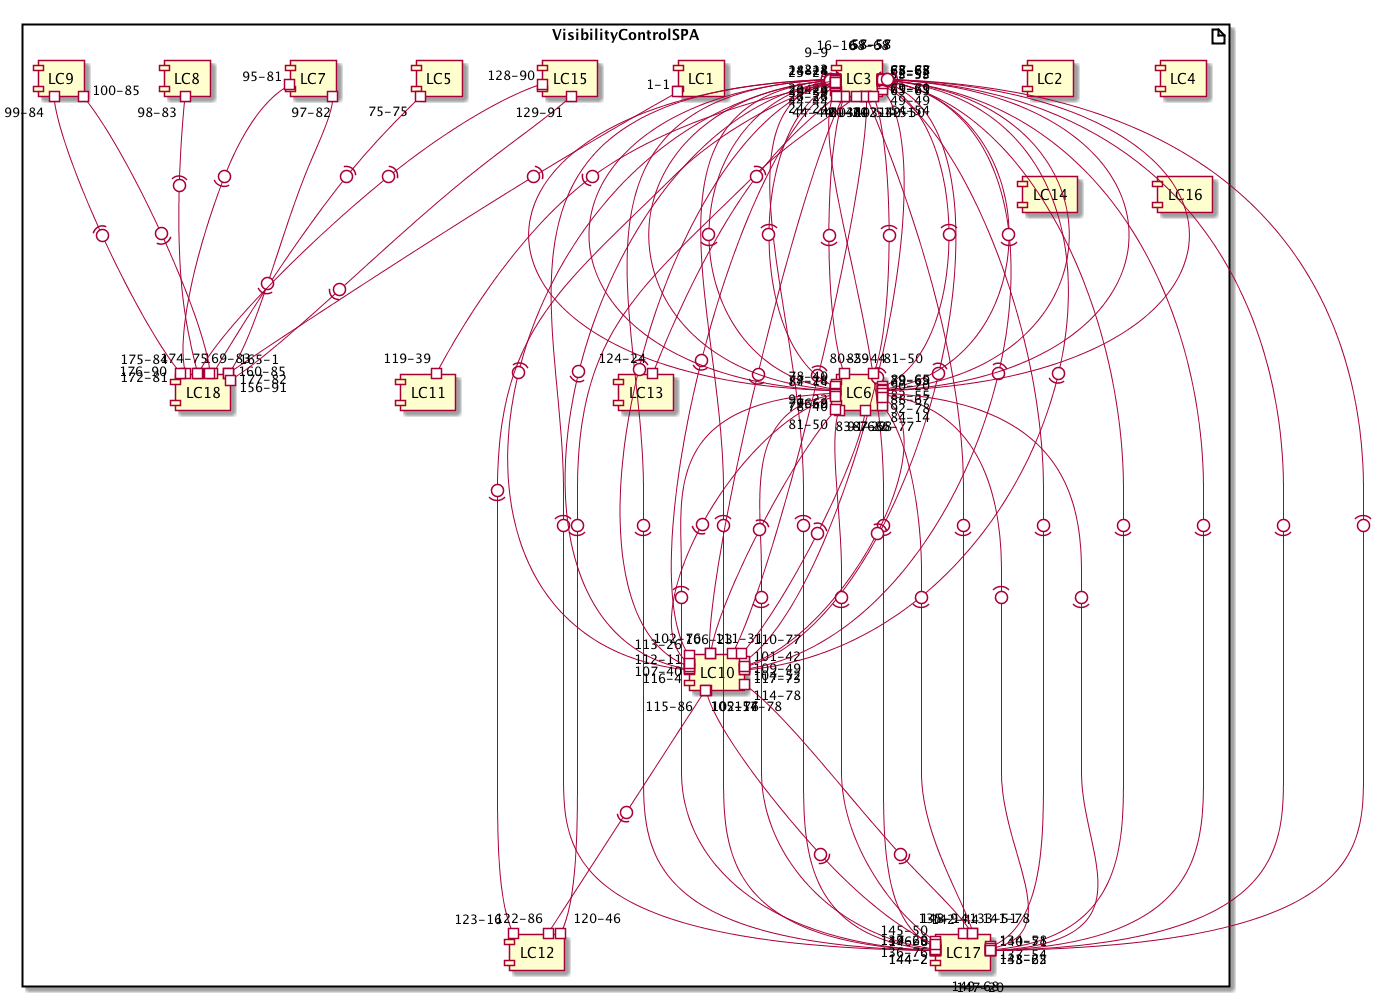
\includegraphics[width=1\linewidth]{figure/results/visualization_1.png}
\caption{Automated visualization prototype}
\label{fig:visualization_one}
\end{figure}

However, there are some limitation of PlantUML. One of the limitation is that the tool does not allow users to move any components once they are rendered from textual description. This makes quite a big impact to our visualization since the sub-system has a large number of artifacts.\\

On the other hand, this proves our idea that visualizing every components and ports is not a good practice. Having a visualization of a complete system provides only an overview of the system, and not all stakeholders who might want to see.

\subsection{Final version of the automated visualization}
\label{RE:final_version_of_the_automated_visualization}
\begin{figure}[H]
\centering
\captionsetup{justification=centering}
\vspace{0cm}% Adjust vertical spacing here
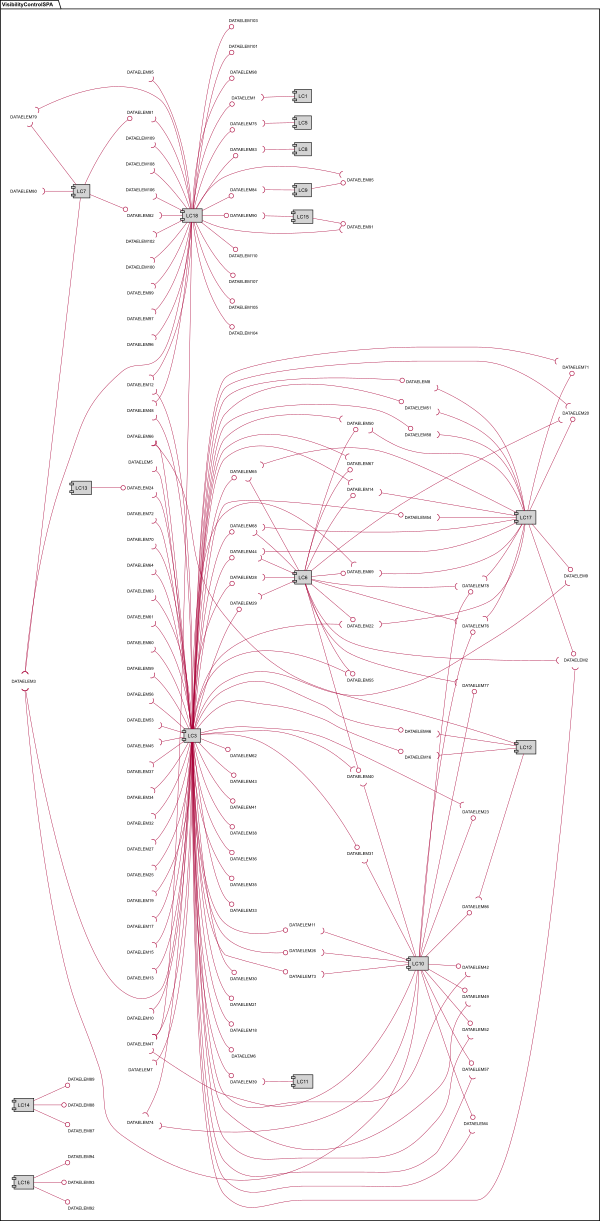
\includegraphics[width=0.7\linewidth]{figure/results/visualization_2.png}
\caption{Final version of the automated visualization}
\label{fig:visualization_final}
\end{figure}


\section{Results from the coding}
\label{RE:results_from_the_coding}
\todo{result from the coding}

\section{Categories of the needs of stakeholders}
\todo{results of each category}